\subsection{Methodology}
Unlike other resources such as CPU and RAM, which are statically divided between the tenants 
based on instance type, network bandwidth is shared among the different co-tenants without a fixed
specification of the expected bandwidth per tenant. Typically, for instances with 16 vCPUs or fewer, 
AWS specifies the bandwidth upper bound, e.g., "Up to 10 Gbps" \cite{network_bandwidth}. However, these 
instances still have a baseline bandwidth. A network I/O credit mechanism 
allows the instance to use burst bandwidth for a short period, ranging from 5 to 60 minutes,
depending on the instance type \cite{network_bandwidth}. \\
Bandwidth throttling for smaller instances takes at least 5 minutes to be enforced, during which the instance
has access to 10 Gbps burst bandwidth. We conduct our experiments in this time window. It is particularly 
interesting to observe the extent of the network degradation in comparison to the baseline bandwidth 
for each instance size.  \\
For network I/O stress, we used iPerf3 \cite{iperf}, a tool that benchmarks network 
bandwidth. It supports multiple protocols and can measure TCP, UDP, and SCTP 
throughput. iPerf3 probes the maximum achievable network bandwidth by transmitting a large number 
of packets until the thoughput's upper bound is reached. The tool requires two nodes — a 
server and a client. Our benchmark measured the 
maximum UDP throughput. We chose UDP in order to avoid congestion 
effects introduced by TCP congestion control, which can reduce measured throughput even
when additional bandwidth is available. \\
To quantify throughput degradation caused by contention between the different tenants, 
we conducted the following experiment. 
\begin{figure}[H]
  \centering
  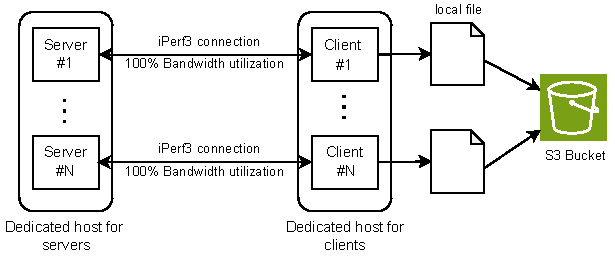
\includegraphics[width=14.5cm, height=6.25cm]{figures/netexp}
  \caption{Throughput contention experiment}
  \label{fig:netexp}
\end{figure}
\noindent
We deployed two dedicated hosts: one hosting the iPerf3 client instances and the other hosting the
corresponding server instances.
We incrementally added client nodes that fully utilized their bandwidth 
through iPerf3 connections with their paired servers. Each client continuously recorded its measured 
throughput to a local log file. We implemented a Python script that computes the average of the 20 
recent data points in the log file and appends the result to a separate output file. 
After each client was deployed, the script was executed across all client nodes using the Distexprunner 
tool. At the end of the experiment, all the output files from the clients were uploaded to an S3 bucket 
for further analysis. \\
Single flow traffic is limited to 5 Gbps, for instances residing in different cluster groups. This is 
the case for the clients and servers since they are placed on different dedicated hosts.   
To bypass this limitation, we established two client connections using the \textit{-P} 
option in the iPerf3 tool. Additionally, the command duration was set  
to 3600 seconds (using the \texttt{-t} option) to ensure steady-state network performance 
without fluctuations caused by repeatedly calling the command. \\
All the VMs were provisioned in the same availability zone and resided
in the same Virtual Private Cloud as mentioned in the \nameref{chapter:infra} chapter. 
